\section{统计推断与实验结果接口}\label{sec:5-10}

在在束 $\gamma$ 谱学分析中，研究人员经历了探测器物理响应（第~5.2~节）、数字波形滤波（第~5.3~节）、高精度定时（第~5.4~节）、硬件活时间与符合选择（第~5.5~节）、符合矩阵与能级拓扑构建（第~5.6~节）、角分布与偏振反演（第~5.7~节）以及微观寿命测量（第~5.8~节）的全流程处理。最终，这些宏观测量必须被综合转化为原子核微观结构的确定物理量——能级激发能 $E_x$、自旋宇称 $I^\pi$、多极混合比 $\delta$、能级平均寿命 $\tau$ 以及绝对电磁约化跃迁几率 $B(XL)$。

然而，由离散计数直方图到连续物理参数的提取并非简单的代数代入，而是一个面临多重不确定度耦合的统计推断反问题。若在分析中机械套用高斯近似或简单忽略系统协方差，容易产生严重的推断失真：其一，在角分布二次反演产生多解双峰、或者微弱谱线处于物理非负边界（$B(XL) \ge 0$）附近时，盲目套用线性误差传播（$\mathbf{J} \mathbf{V} \mathbf{J}^T$）或标准渐近 Wilks 定理，会导致置信区间侵入非物理负值区，或者虚假排除相容解分支；其二，混淆不同测量通道的系统误差与统计涨落，在模型与实验存在微小偏离时轻率宣称发现了新物理。本节构建面向在束谱学的前向测量统计模型，阐明非独立计数似然与非线性协方差传递机制，深入剖析高斯正则性破缺下的轮廓似然与 Feldman-Cousins 物理边界区间构建方法，严格区分统计与系统误差的因果属性，并最终确立标准化的核结构实验结果数据接口。

\subsection{前向测量模型与非独立计数似然}\label{subsec:5-10-1}

在统计物理学中，严谨的实验推断应当建立在前向生成模型（Forward Measurement Model）的基础之上。设系统待求解的微观核结构物理参数集合为 $\boldsymbol{\theta}$（如各能级 $B(E2)$、$B(M1)$、寿命 $\tau$ 及混合比 $\delta$），影响观测但非直接研究目标的伴随扰动参数（Nuisance Parameters，如探测器绝对效率曲线拟合参数、偶然符合归一化因子 $a$、衬底停止本领经验修正因数及侧向馈入时间分布参数）集合记为 $\boldsymbol{\nu}$。

在束实验中，探测器阵列记录的原始能谱由离散事件累积而成。必须明确：离散分箱或事件级记录本身并不自动保证各能量仓计数服从相互独立的泊松分布。各通道计数服从条件独立泊松分布属于分箱近似模型，其物理前提要求满足单通道互斥分类或采用恰当的事件级似然；即使底层复合核反应可近似为泊松点过程，单次核退激仍可能同时发射多个级联光子（多重性 $M_\gamma > 1$），在未做符合拓扑分离时会在不同能量仓之间引入事件级相关。低的每束团反应概率本身不足以证明泊松过程，还需检查束流统计和事件独立性。固定总数并按互斥类别分类时可采用多项模型；硬件容量限制则可能引入停止规则、死时间或选择偏差，需按实际记录过程建模。此外，完整的实验联合似然函数不仅包含信号与连续本底能谱的计数似然，还可纳入来自带外平坦区的背景控制样本以及辅助测量约束。当各辅助标定测量相互条件独立时，辅助项可写作独立概率密度之积；若辅助测量本身存在相关性，则须采用联合概率密度 $p_{\mathrm{aux}}(\mathbf{a} \mid \boldsymbol{\nu})$~\cite{book-zhu-probability-statistics-in-physics, book-behnke-data-analysis-hep, baker-cousins-1984-histogram-fits}：
\begin{equation}\label{eq:5-10-poisson-likelihood}
\mathcal{L}(\boldsymbol{\theta}, \boldsymbol{\nu} \mid \mathbf{n}, \mathbf{a}) = \left[ \prod_{k=1}^K \frac{\mu_k(\boldsymbol{\theta}, \boldsymbol{\nu})^{n_k} e^{-\mu_k(\boldsymbol{\theta}, \boldsymbol{\nu})}}{n_k!} \right] \times p_{\mathrm{aux}}(\mathbf{a} \mid \boldsymbol{\nu}),
\end{equation}
其中 $\mu_k(\boldsymbol{\theta}, \boldsymbol{\nu}) = Y_{\gamma, k}(\boldsymbol{\theta}, \boldsymbol{\nu}) + B_k(\boldsymbol{\nu})$ 为第 $k$ 仓的理论预期计数，$\mathbf{a}$ 为辅助标定观测量，$p_{\mathrm{aux}}(\mathbf{a} \mid \boldsymbol{\nu})$ 为其对应的辅助测量联合概率密度。

前向生成模型式~\eqref{eq:5-10-poisson-likelihood} 明确了从微观物理参数到宏观计数的因果正向映射。与传统启发式峰面积提取相比，它具有以下特性：
\begin{enumerate}
\item 统一表征共享扰动参数引入的相关性：
当不同能量的峰共处于同一测量体系中时，它们对某些全局参数（如总探测时间、绝对效率刻度或探测器死时间因子）的依赖具有强关联。联合似然将这些共性因子作为共享扰动参数 $\boldsymbol{\nu}$ 统一处理，能够定量描述由参数不确定度诱导的协方差；而对多光子事件聚类等底层物理相关性，则需进一步通过事件级联合似然或符合矩阵模型单独表征。
\item 比值中心值丢弃了原始似然形状：
在实验文献中，常将测量结果压缩报告为单峰面积比值（如相对光子强度比或 DCO 强度比）。仅凭比值的中心值与一阶对称误差，无法还原多维空间中由于泊松涨落与效率非线性传递引起的非对称似然曲面。
\end{enumerate}

\subsection{非线性误差传递、Jacobian矩阵与协方差网络}\label{subsec:5-10-2}

当从中间实验观测向量 $\mathbf{x}$（如净峰面积 $A_\gamma$、门选比值、寿命 $\tau$、转换系数 $\alpha_{\mathrm{IC}}$）向最终物理参数向量 $\mathbf{y} = \mathbf{g}(\mathbf{x})$（如绝对 $B(E2)$ 几率）转换时，普遍采用基于一阶 Taylor 展开的线性化误差传播：
\begin{equation}\label{eq:5-10-covariance-prop}
\mathbf{V}_y \approx \mathbf{J} \mathbf{V}_x \mathbf{J}^T,
\end{equation}
其中 $\mathbf{J}$ 为函数的一阶偏导数 Jacobian 矩阵，元素满足 $J_{ik} = \frac{\partial g_i}{\partial x_k}$，$\mathbf{V}_x$ 为输入参量的协方差矩阵。对任一标量输出物理量 $y_i$，其总方差展开式为：
\begin{equation}\label{eq:5-10-var-sum}
\sigma_{y_i}^2 \approx \sum_k J_{ik}^2 \sigma_{x_k}^2 + 2 \sum_{k < l} J_{ik} J_{il} \mathrm{Cov}(x_k, x_l).
\end{equation}

在核物理反演实践中，必须严格审查式~\eqref{eq:5-10-var-sum} 的适用边界（朱永生 2006 第 3 章 §3.9，印刷第 67--70 页，PDF 第 83--86 页~\cite{book-zhu-probability-statistics-in-physics}; Bonamente 2022 第 5 章 §5.2，印刷第 83--87 页，PDF 第 103--107 页，例 5.3~\cite{book-bonamente-statistics-scientific-data}）：
\begin{itemize}
\item 必须保留非零协方差项：
在一阶展开下，当输入参量 $x_k$ 与 $x_l$ 统计不相关（即协方差 $\mathrm{Cov}(x_k, x_l) = 0$）或交叉项代数相消时，总方差才退化为简单的对角平方和 $\sigma_{y_i}^2 = \sum_k J_{ik}^2 \sigma_k^2$。必须明确：不相关性（协方差为零）弱于统计独立性；协方差为零并不自动意味着输入变量相互独立，但在关于均值的一阶 Taylor 展开中，不相关性已足以使交叉协方差项在方差求和中消失。
在在束谱学中，必须清晰区分原始解谱净峰面积 $A_i$（计数）与经效率及活时间校正后的跃迁强度 $I_i = A_i / (\varepsilon(E_i) \cdot \mathrm{LT})$：其中 $\mathrm{LT} \in (0, 1]$ 为无量纲的单探测器活时间份额（Live-Time Fraction），该因式分解假定了探测效率与活时间测量相互独立且信号无时间相关丢失；当处理多探测器符合测量时，正如第~5.5~节所述，联合符合接受度受通道间死时间相关性约束，不能简单拆解为各单道独立效率与活时间的标量积。原始峰面积的拟合协方差 $\mathbf{V}_A$ 源自多高斯解谱或背景扣除（紧密重叠峰通常呈现负相关，但复杂的共同连续本底可能改变相关符号；远离孤立峰近乎零相关）；而经校正后的跃迁强度 $I_i$ 则额外引入了共享探测效率曲线拟合参数的协方差传递。共享全局效率参数在不同能量区间可能引入正协方差或负协方差（取决于效率参数化曲线的局域斜率与曲率），不能笼统假定所有通道间协方差必为正，亦不能在非多项分布情形下断言分支协方差必为负。无声明地丢弃协方差项会严重歪曲最终跃迁几率的总不确定度。
\item 非线性强曲率与代入估计量界限：
对于非线性映射 $\mathbf{g}(\mathbf{x})$，式~\eqref{eq:5-10-covariance-prop} 仅是一阶线性近似。正如第~5.6~节所指出的，对于净计数 $S = P - aR$，在固定 $a$ 与独立泊松条件下理论总体方差为 $\mathrm{Var}(S) = \mu_P + a^2 \mu_R$, 而实验计算中的 $P + a^2 R$ 属于样本代入估计量 $\widehat{\mathrm{Var}}(S)$。当函数具有强非线性曲率（如 $B(E2) \propto E_\gamma^{-5} \tau^{-1}$ 且相对误差较大时），一阶高斯展开可能不足以描述均值、方差或尾部。当解析误差传播由于高度非线性或多峰结构失效时，可以通过对输入物理量的联合分布进行蒙特卡罗抽样，将样本代入非线性转换模型 $\mathbf{g}(\mathbf{x})$ 得到输出参数的前向推演分布（Pushforward Distribution）。必须明确：这种前向抽样反映的是测量误差在外推变换下的统计传播，仅当输入样本本身已经直接来自于相应的条件后验分布时，输出样本的经验直方图才构成合法的参数后验分布；仅仅在输入端形式化附加一个先验分布并不足以使前向抽样等同于严密的贝叶斯后验推断。
\end{itemize}

\subsection{高斯正则性破缺：多峰似然、物理边界与Feldman-Cousins构建}\label{subsec:5-10-3}

传统统计学常假定参数估计量渐近服从正态高斯分布。渐近 Wilks 定理（Wilks 1938; 朱永生 2006 第 12 章 §12.2.2，印刷第 394--398 页，PDF 第 410--414 页~\cite{book-zhu-probability-statistics-in-physics}; Behnke 等 2013 第 2 章 §2.3，印刷第 37--38 页，PDF 第 55 页~\cite{book-behnke-data-analysis-hep}）指出：在零假设处于参数空间内部（无边界效应）且大样本正则条件成立的极限下，对 $m$ 个感兴趣物理参数（Parameters of Interest）进行检验的轮廓似然比统计量 $-2\Delta\ln\lambda(\boldsymbol{\theta})$ 渐近服从自由度等于 $m$ 的 $\chi^2$ 分布，即自由度仅由被检验的物理参数维数 $m = \dim(\boldsymbol{\theta})$ 决定，而不包含被剖面优化消除的伴随扰动参数（Nuisance Parameters）维数。对于单参数检验（$m=1$），双侧 $1\sigma$ 对应 $\Delta\chi^2 = 1.0$，双侧 $95\%$ 置信度对应 $\Delta\chi^2 = 3.84$。
在内部正则点和选定分支的局部高斯近似中，曲率可用于估计协方差。下式中的目标函数应已对伴随参数作剖面优化；也可以先对完整自由参数求Hessian并取其逆矩阵中的相应协方差子块。必须明确 Hessian 矩阵的目标函数定义：若采用负对数似然函数 $F_1(\boldsymbol{\theta}) = -\ln\mathcal{L}$，其二阶导数矩阵（观测 Fisher 信息阵）为 $\mathbf{H}_1 = \nabla^2(-\ln\mathcal{L})$，协方差矩阵近似为 $\mathbf{V}_{\boldsymbol{\theta}} \approx \mathbf{H}_1^{-1}$；若采用检验统计量形式 $F_2(\boldsymbol{\theta}) = -2\ln\mathcal{L}$，其 Hessian 矩阵为 $\mathbf{H}_2 = \nabla^2(-2\ln\mathcal{L}) = 2\mathbf{H}_1$，对应的协方差矩阵近似为 $\mathbf{V}_{\boldsymbol{\theta}} \approx 2 \mathbf{H}_2^{-1}$，推导与编程实现中不可遗漏系数 2。若伴随参数已被轮廓极小化消除，二阶导数反映的是轮廓曲率（Profile Curvature）。
同时必须注意：轮廓似然曲线本身并不自动产生具备精确置信覆盖的置信区间。轮廓似然比区间的置信水平保证依赖于其渐近卡方极限；在有限小样本、多峰或边界附近，精确的置信覆盖必须依赖于对参考分布的构建，例如通过严格的 Neyman 接受带构造、小样本下的离散精确枚举或蒙特卡罗校准获取经验参考分布。在真实的在束核谱学分析中，高斯正则性条件（Gaussian Regularity）常面临以下物理局限：
\begin{enumerate}
\item 多极混合比 $\delta$ 反演的双根多解（Multi-Root Degeneracy）：
在角分布 $W(\theta)$ 或 DCO 强度比的二次有理拟合中，由于二次方程的代数结构，似然曲面常呈现两个分离的极小值峡谷（见图~\ref{fig:5-10-inference-profile}(a)）。在每一个局部极小值附近，局域二阶导数展开（轮廓曲率）可以给出该分支内的局域有效误差；但在全局统计推断中，必须完整报告相容的两个孤立解分支，不能将多峰曲面强行用单高斯抛物线拟合，更不能随意丢弃第二解分支。
\item 物理边界截断与 Feldman-Cousins 统一方法：
核跃迁辐射几率具有严格的物理非负边界（如 $B(E2) \ge 0$、寿命 $\tau \ge 0$）。当微弱谱线由于本底统计下涨落导致无约束极大似然估计量出现负值（$\widehat{\mu} < 0$）时，标准双侧高斯置信区间会导致区间侵入非物理负值区与物理域取交集后还可能得到空集；而若实验人员事后根据估计值正负自行决定报告单边上限还是双边区间（Flip-Flopping），会导致真实的覆盖率严重低于名义置信水平（Undercoverage）。
一种预先固定似然比排序、避免事后翻转报告规则的方法是 Feldman-Cousins 统一方法（Feldman \& Cousins 1998; 朱永生 2006 专著第 11 章 §11.2 似然比顺序求和方法，印刷第 377--379 页，PDF 第 393--395 页，式 (11.2.2)--(11.2.4)~\cite{book-zhu-probability-statistics-in-physics}; Behnke 等 2013 专著第 4 章 §4.3，印刷第 122--123 页，PDF 第 138--139 页 Table 4.2~\cite{book-behnke-data-analysis-hep}）：该方法基于广义似然比排序原理 $R(n \mid \mu) = P(n \mid \mu) / P(n \mid \hat{\mu}_{\mathrm{phys}})$（其中 $\hat{\mu}_{\mathrm{phys}} = \max(0, \hat{\mu})$ 为物理受限极大似然估计），对声明的生成模型（如已知本底 $b$ 下的泊松信号）在参数空间上逐点构造 Neyman 接受带并进行反演。必须明确：对于离散泊松计数，接受带的端点随整数计数跳跃变化，通常表现出保守的阶梯状过覆盖（Over-coverage）；Feldman-Cousins 方法绝非简单在连续轮廓似然曲线上截取 $\Delta\chi^2 = 2.71$（后者仅为一维渐近单侧 $95\%$ 正态标尺，见图~\ref{fig:5-10-inference-profile}(b) 展示），更不能在任意包含复杂伴随参数剖面优化的情形下假定普适平滑覆盖。当报告置信区间与上限时，必须明确声明所选取的推断构型、置信水平、排序准则以及伴随参数的处理流程。
\end{enumerate}

为直观展示上述高斯破缺机制及规范统计处理方法，图~\ref{fig:5-10-inference-profile} 给出了基于标准教学模型的合成多峰剖面与同一高斯观测下的受限似然对比图。

\begin{figure}[!htbp]
\centering
%
  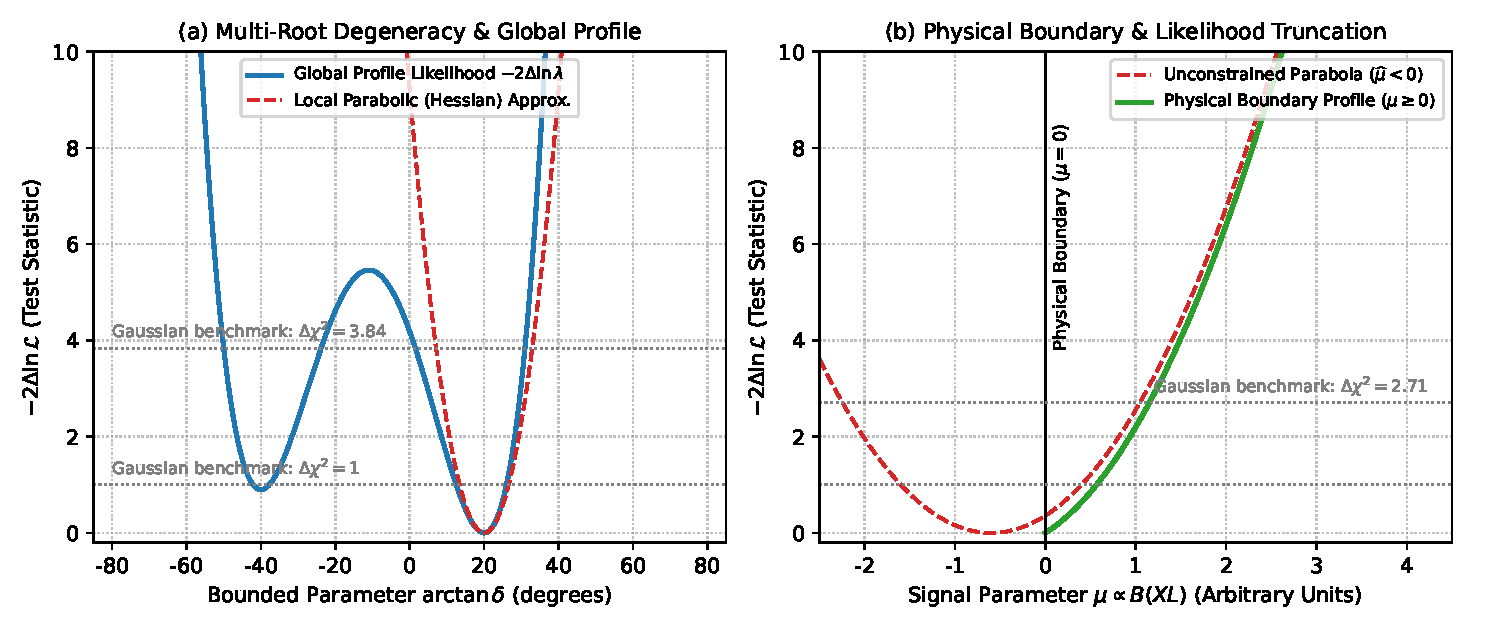
\includegraphics[width=0.92\textwidth]{Img/inference-profile-likelihood-boundary.pdf}%
\caption[核谱学高斯正则性破缺与统计推断模型对比]{核谱学高斯正则性破缺与统计推断模型对比（规范教学模型）。(a) 展示多极混合比 $\delta$ 在有界坐标 $\arctan\delta$ 上的整体轮廓似然曲线（实线），呈现清晰的双极小值结构；虚线是该合成函数在右侧极小点处的实际二阶Taylor近似，说明对称高斯假设完全丢弃了第二解分支；(b) 展示信号参数处于物理非负边界（$\mu \ge 0$）时的轮廓似然曲线：虚线为允许负值的无约束剖面（极小值处于统计负涨落点 $\widehat{\mu} < 0$），绿色实线展示了严格定义在物理非负定义域 $\mu \ge 0$ 上且归一至受限极大值 $\hat{\mu}_{\mathrm{phys}} = 0$ 的轮廓似然剖面，受限曲线由同一观测 $\widehat\mu=-0.6$ 的高斯对数似然减去其物理最优点处的值构成；约束只改变参考极大值，不将观测均值重置为零（图中1、3.84与2.71水平均仅作一参数高斯标尺，未给该合成多峰例校准覆盖率；$\Delta\chi^2 = 2.71$ 虚线仅表示一维高斯渐近单侧 $95\%$ 标尺，不代表通用的 Feldman-Cousins 覆盖结果；严格的 Feldman-Cousins 统一区间构建基于对具体生成模型的似然比排序 Neyman 接受带反演，离散泊松计数呈现阶梯状过覆盖，不可直接等同于连续曲线截断）。注意此处为规范教学模型展示，非特定未知实验测量拟合）。}
\label{fig:5-10-inference-profile}
\end{figure}

针对图~\ref{fig:5-10-inference-profile} 所示的非正则场景，在数据分析中应规范应用以下推断方法：
\begin{itemize}
\item 轮廓似然方法（Profile Likelihood）：
对于包含众多扰动参数 $\boldsymbol{\nu}$ 的复杂模型，通过在固定感兴趣物理参数 $\boldsymbol{\theta}$ 的条件下对所有扰动参数进行受限极大似然优化（$\hat{\hat{\boldsymbol{\nu}}}(\boldsymbol{\theta})$），构建单变量或双变量的轮廓似然比检验统计量：
\begin{equation}\label{eq:5-10-profile-likelihood}
\lambda(\boldsymbol{\theta}) \equiv \frac{\mathcal{L}(\boldsymbol{\theta}, \hat{\hat{\boldsymbol{\nu}}}(\boldsymbol{\theta}))}{\mathcal{L}(\hat{\boldsymbol{\theta}}, \hat{\boldsymbol{\nu}})}.
\end{equation}
轮廓似然方法自动将扰动参数的统计不确定度沿极小化路径向外投影，从而在输出曲线上产生反映非线性与关联效应的非对称置信区间。必须注意：仅当样本量充足且处于内部正则区时，$-2\ln\lambda(\boldsymbol{\theta})$ 才渐近服从自由度为 $\dim(\boldsymbol{\theta})$ 的 $\chi^2$ 分布；在小样本或边界情形下，必须结合蒙特卡罗校准获取经验参考分布。
\item 蒙特卡罗抽样与推演分布（Monte Carlo Pushforward）：
当解析误差传播由于高度非线性或多峰结构失效时，可以通过对输入物理量的联合分布进行蒙特卡罗大样本抽样，将样本代入非线性转换模型 $\mathbf{g}(\mathbf{x})$ 得到输出参数的前向推演分布。必须明确：这种前向抽样反映的是测量误差的传播分布，仅当输入样本本身已经直接来自于相应的条件后验分布时，输出分布方可作为贝叶斯后验概率密度解释。
\end{itemize}

\subsection{系统误差、统计涨落与模型假象的甄别}\label{subsec:5-10-4}

在科学写作与理论比对中，必须严格区分两类性质根本不同的实验不确定度来源：
\begin{enumerate}
\item 统计涨落误差（Statistical Uncertainty）：
源于核衰变发射与探测器电荷电离过程的本征微观量子随机性。在渐近独立平稳泊松极限下，计数的绝对统计标准差按 $\sigma \sim \sqrt{N_{\mathrm{counts}}}$ 增长，而相对统计精度按 $1/\sqrt{N_{\mathrm{counts}}}$ 改善；通过延长束流照射时间可以在统计涨落层面提高信噪比。
\item 系统不确定度（Systematic Uncertainty）：
源于物理模型假设偏差、仪器刻度基准偏移以及探测环境的全局畸变。系统不确定度并不必然在所有探测通道呈现相同方向，且不能通过简单延长机时来消除；部分系统偏差可通过增加辅助刻度实验予以缩小。在低能核物理在束谱学中，典型的系统误差来源包括：
\begin{itemize}
\item 探测器绝对全能峰效率曲线的参数化拟合不确定度及其跨能区协方差传递；
\item 第~5.8~节 DSAM 谱形拟合中所采用的固体衬底微观电子/核停止本领理论模型参数差异（如 SRIM 与 Northcliffe-Schilling 唯象参数之间的系统离散）；
\item 反应靶实际厚度、同位素纯度与反冲慢化介质密度的实验测量公差；
\item 符合时间窗口截断与偶然本底扣除归一化比例因子 $a$ 的拟合或标定不确定度。
\end{itemize}
\end{enumerate}

在核结构科学推断中，提出一项新的物理模式候选（如手征双重带或摆动激发候选），需要明确说明其实验指征、模型依赖性以及当前的观测边界；而确证一项新的集体模式主张，则必须对已知的仪器效应、数据处理假象以及常规竞争机制（如准粒子顺排带交叉、形状共存或 $\gamma$ 振动）开展系统的敏感性检验与排他性评估。研究人员应重点核查以下竞争性仪器与方法学因素：
\begin{enumerate}
\item 观察到的弱支路偏离是否完全处于探测器全能峰效率曲线与偶然相加校正的系统误差包络之内；
\item 提取的能级寿命是否受到了未被观测的慢速侧向馈入（Side-Feeding）或未知同核异能态的滞后卷积（见第~5.1~节与第~5.8~节）；
\item 角分布多极混合比反演中是否存在另一个完全相容的数学解分支尚未被排除（见第~5.7~节）；
\item 微观理论模型本身是否由于冻结了准粒子对齐、采用了单态平均场惯量参数或忽略了 $\gamma$ 自由度的大振幅涨落而导致模型自身预测失真。
\end{enumerate}
确证一项新的集体模式主张需要开展相称的排他性检验与系统敏感性核查；而探索性的物理模式候选则可以基于初步观测指征提出，并清晰声明其灵敏度边界与待验条件。

\subsection{核结构实验结果标准输出数据接口}\label{subsec:5-10-5}

为了将第 5 章所建立的在束谱学因果链条严密固化为可供理论模型（第 2、3、4 章）直接检验的高保真实验结果，本节确立了一套标准化的核结构实验输出数据接口。

在正式的学位论文与学术成果报告中，任何一条关于能级与电磁强度的陈述，均应在数据表中完整列出其初末态量子数、观测谱学量、中间修正因子、反演物理量及其不确定度分解。表~\ref{tab:5-10-transitions-template}、表~\ref{tab:5-10-strengths-template} 与表~\ref{tab:5-10-method-cov-template} 分别给出了跃迁观测、强度反演与协方差网络记录的规范格式模板。表内数值仅为教学设置，用来说明字段、单位和多解分支的报告方法，不对应用户的实验测量。

\begin{table}[!htbp]
\centering\small\setlength{\tabcolsep}{2pt}
\caption{低能核结构在束谱学特征跃迁与探测观测数据接口模板（格式规范模板；各条目展示数据字段结构与单位约定；对于存在多解相容分支的多极混合比，完整并列报告各候选根分支）。}
\label{tab:5-10-transitions-template}
\begin{tabular}{@{}>{\raggedright\arraybackslash}p{.075\textwidth}>{\raggedright\arraybackslash}p{.12\textwidth}>{\raggedright\arraybackslash}p{.12\textwidth}>{\raggedright\arraybackslash}p{.11\textwidth}>{\raggedright\arraybackslash}p{.13\textwidth}>{\raggedright\arraybackslash}p{.10\textwidth}>{\raggedright\arraybackslash}p{.20\textwidth}@{}}
\toprule
\shortstack[l]{跃迁\\标记} & \shortstack[l]{初态\\$E_i(I_i^\pi)$} & \shortstack[l]{末态\\$E_f(I_f^\pi)$} & \shortstack[l]{能量\\$E_\gamma$} & \shortstack[l]{相对强度\\$I_\gamma$} & \shortstack[l]{多极\\$XL$} & \shortstack[l]{混合比\\$\delta(E2/M1)$} \\
& (keV) & (keV) & (keV) & (光子产额) & & (KS 约定) \\
\midrule
$\gamma_1$ & $E_1\,(2_1^+)$ & $0\,(0_1^+)$ & $E_{\gamma 1}$ & $100$ (基准) & 纯 $E2$ & $\delta^{-1} = 0$ \\
$\gamma_2$ & $E_2\,(4_1^+)$ & $E_1\,(2_1^+)$ & $E_{\gamma 2}$ & $35.2(6)$ & 纯 $E2$ & $\delta^{-1} = 0$ \\
$\gamma_3$ & $E_3\,(2_2^+)$ & $E_1\,(2_1^+)$ & $E_{\gamma 3}$ & $18.4(4)$ & $M1+E2$ & 根 1: $-0.35(4)$ \\
& & & & & & 根 2: $+1.59(8)$ \\
$\gamma_4$ & $E_3\,(2_2^+)$ & $0\,(0_1^+)$ & $E_{\gamma 4}$ & $6.2(3)$ & 纯 $E2$ & $\delta^{-1} = 0$ \\
\bottomrule
\end{tabular}
\end{table}

\begin{table}[!htbp]
\centering\small\setlength{\tabcolsep}{2pt}
\caption{微观核态寿命、分支比与绝对电磁跃迁几率数据接口模板（格式规范模板；各能级自成独立组态行，各分支总和在同母态内归一；对于存在混合比双根的多极跃迁，同时并列计算两组相容的 $B(M1)$ 与 $B(E2)$ 几率）。}
\label{tab:5-10-strengths-template}
\begin{tabular}{@{}>{\raggedright\arraybackslash}p{.11\textwidth}>{\raggedright\arraybackslash}p{.10\textwidth}>{\raggedright\arraybackslash}p{.10\textwidth}>{\raggedright\arraybackslash}p{.13\textwidth}>{\raggedright\arraybackslash}p{.12\textwidth}>{\raggedright\arraybackslash}p{.16\textwidth}>{\raggedright\arraybackslash}p{.16\textwidth}@{}}
\toprule
\shortstack[l]{能级\\$E_i$} & \shortstack[l]{寿命\\$\tau$} & \shortstack[l]{测时\\方法} & \shortstack[l]{退激\\跃迁} & \shortstack[l]{总分支比\\$b_{\mathrm{tot}}$} & $B(E2)\downarrow$ & $B_\mu(M1)\downarrow$ \\
(keV) & (ps) & & & (含内转换) & ($e^2\text{fm}^4$) & ($\mu_N^2$) \\
\midrule
$E_1\,(2_1^+)$ & $\tau_1$ & RDDS & $\gamma_1 \to 0_1^+$ & $1.000$ & $B(E2)_1$ & --- \\
\midrule
$E_2\,(4_1^+)$ & $\tau_2$ & RDDS & $\gamma_2 \to 2_1^+$ & $1.000$ & $B(E2)_2$ & --- \\
\midrule
$E_3\,(2_2^+)$ & $\tau_3$ & DSAM & $\gamma_3 \to 2_1^+$ & $b_{31}$ & $B(E2)_{31}^{(1)}$ & $B_\mu(M1)_{31}^{(1)}$ \\
& & & & & $B(E2)_{31}^{(2)}$ & $B_\mu(M1)_{31}^{(2)}$ \\
& & & $\gamma_4 \to 0_1^+$ & $b_{30}$ & $B(E2)_{30}$ & --- \\
\bottomrule
\end{tabular}
\end{table}

\begin{table}[!htbp]
\centering\small\setlength{\tabcolsep}{2pt}
\caption{核结构实验方法学约束与协方差网络记录规范模板（展示不同观测参量间的统计相关性与报告规范）。}
\label{tab:5-10-method-cov-template}
\begin{tabular}{@{}>{\raggedright\arraybackslash}p{.23\textwidth}>{\raggedright\arraybackslash}p{.20\textwidth}>{\raggedright\arraybackslash}p{.52\textwidth}@{}}
\toprule
参量标识 & 物理对象 / 关联来源 & 规范处理准则与协方差报告口径 \\
\midrule
$\mathrm{Cov}(b_i, b_j)$ & 同一母态各退激分支比 & 总分支归一 $\sum_k b_k = 1$ 给出线性行和约束 $\sum_j \mathrm{Cov}(b_i, b_j) = 0$；在指定固定总数的多项模型下，不同非零分支的协方差为负，零概率分支可给出零协方差，一般情形需由各产额与标定参数的联合协方差向前传递 \\
$\mathrm{Cov}(A_i, A_j)$ & 原始拟合净峰面积 & 由能谱解叠多高斯拟合与本底扣除给出（重叠峰通常呈负相关，但未知共同本底或相加效应可能改变相关符号） \\
$\mathrm{Cov}(I_i, I_j)$ & 效率校正后相对强度 & 由原始面积误差与共享效率刻度参数协方差共同传递，不同能区可能为正或为负 \\
$\delta_1, \delta_2$ & DCO / 角分布反演双根 & 完整保留两组相容候选根（保持 Krane--Steffen 约定数值），分别评估其对后续微观 $B(XL)$ 反演的影响 \\
\shortstack[l]{$\tau_{\mathrm{limit}}$\\$B(XL)_{\mathrm{limit}}$} & 测时灵敏度物理极限 & 明确注明减速截面模型与置信度；多极限联合报告时给出联合覆盖区域 \\
\bottomrule
\end{tabular}
\end{table}

表~\ref{tab:5-10-transitions-template}、表~\ref{tab:5-10-strengths-template} 与表~\ref{tab:5-10-method-cov-template} 直观展示了从谱学实验到物理结果的自洽接口规范：
\begin{itemize}
\item 相对光子强度 $I_\gamma$ 与总跃迁分支比 $b_{\mathrm{tot}}$ 明确分开：表~\ref{tab:5-10-strengths-template} 中的总跃迁分支比 $b_{\mathrm{tot}}$ 包含内转换通道贡献，满足同一母能级所有退激分支和归一 $\sum_k b_{\mathrm{tot}, k} = 1.000$；其对应的纯辐射光子发射份额由 $b_\gamma = b_{\mathrm{tot}} / (1 + \alpha_{\mathrm{IC}})$ 给出，不可将总跃迁分支比 $b_{\mathrm{tot}}$ 与表~\ref{tab:5-10-transitions-template} 中未计内转换的相对光子发射强度 $I_\gamma$ 混同。以最强跃迁归一基准时，标明定义基准（无统计误差）或实测外标误差；
\item 多极混合比 $\delta$ 在偏振未解简并前，完整保留相容的两个数值解分支，并统一采用与第~5.9~节一致的 Krane--Steffen 相位约定；
\item 能级寿命 $\tau$ 清晰标明测量方法（如 DSAM、RDDS 或快定时），在灵敏度之外如实标注确定置信度水平的单边上下限；若声称多项极限具有同时覆盖，应说明联合覆盖构造；仅并列报告边际限时则标明各自置信水平，不能把它们自动当作一个同水平的联合结论；
\item 约化跃迁几率必须明确注明下行（Downwards）定义及量纲单位：电四极采用 $B(E2)\downarrow$（单位为 $e^2\text{fm}^4$ 或 $e^2\text{b}^2$）；磁偶极采用与第~5.9~节实用辐射跃迁几率接口对齐的电磁矩算符约化跃迁几率 $B_\mu(M1)\downarrow$（单位为 $\mu_N^2$）。若采用附录A定义的电荷型磁算符 $\mathcal M_S=\mathcal M_\mu/c$，则有量纲的物理强度满足 $B_S(M1)=B_\mu(M1)/c^2$；分别以 $(\mu_N/c)^2$ 和 $\mu_N^2$ 为单位归一后的数值相同。这里的 $B_S$ 不代表新定义的无量纲自旋强度。各跃迁几率均附带经由式~\eqref{eq:5-10-var-sum} 完整协方差传播的不确定度。
\end{itemize}
必须严肃说明：上述三表中所列条目为展示数据结构规范的教学格式模板，不代表任何未经实测的虚构用户项目数据；针对具体核素（如 $^{130, 131, 133}\mathrm{Ce}$ 或 $^{74}\mathrm{As}$）的实际测量填报，必须完全基于真实实验台账与已公开原始文献定位符逐项核录。

通过本章从探测物理（第~5.2~节）到统计推断接口（第~5.10~节）的层层递进，低能原子核结构在束 $\gamma$ 谱学建立起了一套因果清晰、可追溯的实验测量与数据推断规范，为检验全篇微观形状共存、非轴对称转动动力学与电磁跃迁定则提供了坚实可靠的数据基石。
